%\appendix{}  % Change to appendices if more than one

\appendix
\linespread{1.7}
\chapter*{Appendix}
\linespread{2.0}
\addcontentsline{toc}{chapter}{Appendix}
%%%%%%%%%%%%%%%%%%%%%% A
\renewcommand{\thesection}{A}
\renewcommand{\thesubsection}{A\arabic{subsection}}
\numberwithin{figure}{section}
\numberwithin{table}{section}
\numberwithin{equation}{section}
\renewcommand{\thefigure}{A\arabic{figure}}
\renewcommand{\theequation}{A\arabic{equation}}
\renewcommand{\thetable}{A\arabic{table}}


\linespread{1.7}
\section{Von Karmen Autocorrelation Function}
\linespread{2.0}
%\newrefsection
\label{app:A}

The form of the Von Karman autocorrelation function \citep{frankelFiniteDifferenceSimulations1986} is

\begin{equation}\label{eq:app-A1}
    \Phi_{v, a}(r)=\sigma^{2} \frac{2^{1-v}}{\Gamma(v)}\left(\frac{r}{a}\right)^{v} K_{v}\left(\frac{r}{a}\right)
\end{equation}

\noindent in which $\nu$ is the Hurst component, $a$ is the correlation length, $K_{\nu}$ is the modified Bessel function of order $\nu$, $\Gamma(\nu)$ is the gamma function, and $\sigma^2$ is the variance with Fourier transform:

\begin{equation}\label{eq:app-A2}
    P(k)=\frac{\sigma^{2}(2 \sqrt{\pi} a)^{E} \Gamma(v+E / 2)^{v+E / 2}}{\Gamma(v)\left(1+k^{2} a^{2}\right)}
\end{equation}

\noindent in which $k$ is the wave number and $E$ is the Euclidean dimension.

\clearpage
\floatsetup[figure]{font=sf,style=plain,subcapbesideposition=top}
\begin{figure}[!ht]
    \sidesubfloat[]{\includegraphics[width=0.4\textwidth]{figures/figure_vs30_14a.png}\label{fig:vs30-14a}} \hfil
    \sidesubfloat[]{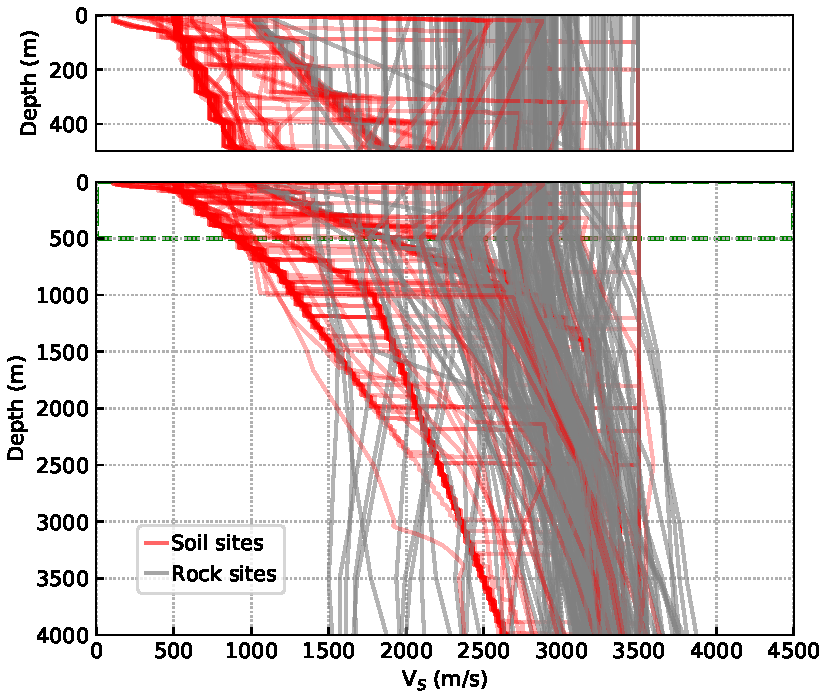
\includegraphics[width=0.45\textwidth]{figures/figure_vs30_14b.pdf}\label{fig:vs30-14b}} % \\[\baselineskip]%
    \caption{ (a) $V_S$ profile sample locations in California. Triangles denote rock sites and circles denote soil sites, and (b) extracted $V_S$ profiles. The top panel zooms into the top 500 m. }
\end{figure}

%%%%%%%%%%%%%%%%%%%%%%%% A (end)


%%%%%%%%%%%%%%%%%%%%%% B
%%%%%%%%%%%%%%%%%%%%%%%% B (end)



%\endrefsection
